
\documentclass{beamer}

\usepackage{graphicx}
\usepackage{epstopdf}
\begin{document}
\title{EE5327 Optimization}   
\author{Sachin Goyal (EE18MTECH11015), \newline Subhra Shankha Bhattacherjee (EE19MTECH01008)} 
\date{\today} 

\frame{\titlepage} 

\section{Section no.1} 
\frame{
4.5 Minimize 
\begin{equation}
 f(x) = -x_{11} - 2x_{12} - 5x_{22}
\end{equation}
subject to
\begin{align}
\label{ch3_lin_mat_ineq_const}
2x_{11} + 3x_{12} + x_{22} &= 7 \\
x_{11} + x_{12} &\geq 1 \\
x_{11}, x_{12}, x_{22} &\geq 0 \\
\begin{pmatrix}
x_{11} & x_{12} \\
x_{12} & x_{22}
\end{pmatrix} & \succeq 0 
\end{align}

by converting the problem into a convex optimization problem in two variables and using graphical plots.
}

\section{Subsection no.1.1  }

\frame{
By converting to two variable convex problem

Minimize
\begin{equation}
9x_{11} + 13x_{12}
\end{equation}
subject to
\begin{align}
\label{ch3_lin_mat_ineq_const}
x_{11} + x_{12} &\geq 1 \\
x_{11}, x_{12} &\geq 0 \\
\begin{pmatrix}
x_{11} & x_{12} \\
x_{12} & x_{22}
\end{pmatrix} & \succeq 0 
\end{align}

}
\section{Graphical Solution} 

\frame{\frametitle{Graphical Solution}
\begin{figure}
\centering
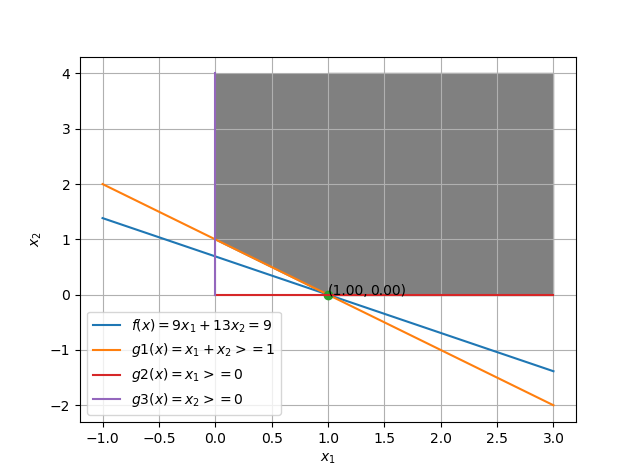
\includegraphics[width=4in]{45.png}
\label{fig.4.1}	
\end{figure}
}

\section{Subsection no.1.2  }

\frame{

We Get:
\begin{align}
\label{}
x_{11} &=1\\
x_{12} &=0
\end{align}

By substituting these values in equation (2)
\begin{align}
\label{}
2x_{11} + 3x_{12} + x_{22} &= 7 
\end{align}
We Get:
\begin{align}
\label{}
x_{11} &=1\\
x_{12} &=0\\
x_{22} &=5
\end{align}
}

\section{Subsection no.1.2  }

\frame{

Our Solution is::
\begin{align}
\label{ch3_lin_mat_ineq_const}
\begin{pmatrix}
1 & 0 \\
0 & 5
\end{pmatrix}
\end{align}


Its Eigenvalues are: 1,5\\
Hence it is a positive semidefinite matrix

\begin{align}
\label{ch3_lin_mat_ineq_const}
\begin{pmatrix}
1 & 0 \\
0 & 5
\end{pmatrix} & \succeq 0 
\end{align}
}

\end{document}